\chapter{Electroweak Theory}
\label{chap:SM}

Developed in the 1960s, the Glashow–Weinberg–Salam theory of the \ac{EW} interaction is regarded by many physicists as the cornerstone of the \ac{SM}. It successfully unified the weak interaction with electromagnetism and postulated the existence of several new particles, all of which were later confirmed by experiments. One of the most important aspects of this theory is the \ew~gauge symmetry, which is discussed in \autoref{sec:Gauge}. The \ew~ symmetry is spontaneously broken through the Higgs mechanism, which is discussed in \autoref{sec:Higgs}. Finally, flavor physics and its connection to the Yukawa interaction is discussed in \autoref{sec:Flavor}. 

\section{Gauge Theory}
\label{sec:Gauge}

Fundamental forces in the \ac{SM} are formulated under a principle known as gauge invariance, where the Lagrangian is invariant under local transformations of gauge groups. Taking \ac{QED} as an example, the local symmetry for a Dirac fermion is,

\begin{equation}
\psi\rightarrow e^{i\alpha(x)}\psi,
\end{equation}

where $\alpha(x)$ is a phase angle defined at each spacetime point, hence the name ``local transformation''. The gauge group associated with this symmetry is $U(1)_{EM}$, where the subscript is a shorthand expression for ``electromagnetism''. Under a local $U(1)_{EM}$ rotation, Equation~\ref{eq:Dirac} can be written as:

\begin{equation}
\begin{split}
\label{eq:QEDGauge}
\mathcal{L}&=-\frac{1}{4}F_{\mu\nu}F^{\mu\nu}+ie^{-i\alpha(x)}\bar{\psi}\gamma^{\mu}\partial_{\mu}e^{i\alpha(x)}\psi-m\bar{\psi}\psi-e\bar{\psi}\gamma^{\mu}(A_{\mu}+\delta A_{\mu})\psi\\
&=\mathcal{L}_{Dirac}-\bar{\psi}\gamma^{\mu}\psi\partial_{\mu}\alpha(x)-e\bar{\psi}\gamma^{\mu}\delta A_{\mu}\psi.
\end{split}
\end{equation}

The gauge invariance requires $\delta A_{\mu}=-\frac{1}{e}\partial_{\mu}\alpha(x)$. This means the photon field transforms as:

\begin{equation}
A_{\mu}\rightarrow A_{\mu}-\frac{1}{e}\partial_{\mu}\alpha(x).
\end{equation}

This behavior of the photon field under gauge transformation cancels out the gauge dependency of the free Dirac Lagrangian, which ensures the gauge invariance of the theory. Therefore, vector bosons such as photons also called gauge bosons, and the associated quantum fields are also known as gauge fields. The Dirac Lagrangian can be re-written as,

\begin{equation}
\label{eq:QEDCov}
\mathcal{L}=-\frac{1}{4}F_{\mu\nu}F^{\mu\nu}+i\bar{\psi}\gamma^{\mu}D_{\mu}\psi-m\bar{\psi}\psi,
\end{equation}

where $D_{\mu}=\partial_{\mu}+ieA_{\mu}$ is known as the gauge covariant derivative. 

The mass term associated to the photon field $\frac{1}{2}m^2A_{\mu}A^{\mu}$ is however not gauge invariant as

\begin{equation}
[A_{\mu}-\frac{1}{e}\partial_{\mu}\alpha(x)][A^{\mu}-\frac{1}{e}\partial^{\mu}\alpha(x)]\neq A_{\mu}A^{\mu}.
\end{equation}

Effectively, this means gauge bosons such as photons must be massless in a gauge invariant theory. As a consequence, a new mechanism, known as the Higgs mechanism, is needed to explain the origin of weak boson masses, which is discussed in the following chapter. 

It should be pointed out that gauge symmetry is not a symmetry of nature. The Noether currents~\cite{Noether1918} associated with local gauge symmetry do not generally correspond to physical observables. Nevertheless, its existence is necessary to regulate the redundant degree of freedom in the Lagrangian using a procedure known as gauge fixing~\cite{SCHWARTZ}. 

\ac{QED} is also known as an abelian gauge theory as the $U(1)$ group operation is commutative, meaning the order of sequential group operations does not affect the final result. Chinese physicist Chen-Ning Yang and his American colleague Robert Mills at Brookhaven first generalized the concept of gauge invariance to the non-abelian Lie group, proposing what's now known as the Yang-Mills theory in 1954~\cite{Yang:1954ek}. Shortly after this work, Yang and his colleague Tsung-Dao Lee suggested parity might be violated in the weak interaction~\cite{Lee:1956qn}, which was later confirmed by the legendary Wu experiment led by Chien-Shiung Wu~\cite{Wu:1957my}. 

Not long after the Wu experiment, physicists understood that only left-handed fermions and right-handed antifermions are involved in weak charged-current interactions. Moreover, the very existence of weak charged-current forced physicists to consider the interaction between photons and weak mediators. This led to many problems in the weak theory, for example, the exchange of photons in $s$-channel $\textsf{e}^{+}\textsf{e}^{-}\rightarrow\textsf{W}^{+}\textsf{W}^{-}$ (shown in Figure~\ref{fig:eeWW}) would lead to divergence at high energy unless there exists a neutral intermediate field that mediates the weak interaction. Hints of the weak neutral current and the interplay between electromagnetism and the weak interaction prompted the efforts by physicists to relate these two forces under the framework of Yang-Mills theory in the early 1960s. 

\begin{figure}[tbh!]
 \begin{center}
 \begin{tabular}{c}
 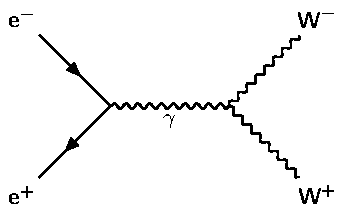
\includegraphics[width=0.6\textwidth]{figures/Part1/SM/eeWW}
 \end{tabular}
 \caption{Representative $s$ channel ee$\rightarrow$WW diagram, mediated by a massless photon field. Without a heavy neutral mediator, such a process would lead to divergence at high energy scales.}
 \label{fig:eeWW}
 \end{center}
\end{figure}

Since fermions with different chiral structures were understood to be treated differently by the weak interaction, it was 
imperative to apply different gauge transformations to left-handed and right-handed fermionic fields. Initial work toward unification was done by American physicist Sheldon Glashow, who proposed the \ew~symmetry in 1961~\cite{Glashow:1961tr}, where $L$ denotes left-handed fields, and Y refers to the quantum number for hypercharge. Under this framework, left-handed components of the Dirac fields are organized into $SU(2)_{L}$ doublet,

\begin{equation}
L_{L}^{j}=\begin{pmatrix}\nu^{j}\\ e^{j}\end{pmatrix}_{L}, Q_{L}^{j}=\begin{pmatrix}u^j\\d^j\end{pmatrix}_{L}, j=1, 2, 3,
\end{equation}

where $\nu^{j}$, $e^{j}$, $u^{j}$, and $d^{j}$ correspond to Dirac fields of neutrino, charged-lepton, up-type quark, and down-type quark, respectively. The right-handed components of the Dirac fields are treated as $SU(2)_{L}$ singlet: $e_{R}^{j}, u_{R}^{j}, d_{R}^{j}$, where neutrino terms are missing as only left-handed neutrinos have been observed in nature. The index $j$ in both doublets and singlets runs over the fermion generations. The left-handed doublets carry $\frac{1}{2}$ weak isospin charge, denoted by $T$. The third component of $T$, denoted by $T_3$, is $\frac{1}{2}$ for neutrinos and up-type quarks, and -$\frac{1}{2}$ for charged-leptons and down-type quarks in the $SU(2)_{L}$ doublets. All right-handed singlets carry 0 weak isospin charge, which prevents them from participating in the weak interaction. 

The \ew~symmetry introduces the following local gauge transformations:

\begin{equation}
\begin{split}
&\Psi_{L}\rightarrow\textsf{exp}[i\hat{T}^{i}\alpha^{i}(x)+i\frac{\hat{Y}}{2}\beta(x)]\Psi_{L},\\
&\Psi_{R}\rightarrow\textsf{exp}[i\frac{\hat{Y}}{2}\beta(x)]\Psi_{R},
\end{split}
\end{equation}

where $\Psi_{L}=\{L_{L}^{j},Q_{L}^{j}\}$, and $\Psi_{R}=\{e_{R}^{j}, u_{R}^{j}, d_{R}^{j}\}$. $\hat{T}^{i}$ and $\hat{Y}$ denotes generators of the $SU(2)_{L}$ and $U(1)_{Y}$ group, respectively. To preserve gauge invariance, two massless gauge fields $W_{\mu}$ and $B_{\mu}$ are introduced. The corresponding gauge covariant derivative can be written as

\begin{equation}
\label{eq:EWCov}
D_{\mu}=\partial_{\mu}-ig\hat{T}^{i}W_{\mu}^{i}-ig^{\prime}\frac{\hat{Y}}{2}B_{\mu},
\end{equation}

where $g$ and $g^{\prime}$ correspond to coupling strengths of the $SU(2)$ and $U(1)$ gauge fields, respectively. The \ew~gauge Lagrangian can therefore be written as:

\begin{equation}
\label{eq:LagGauge}
\mathcal{L}_{gauge}=-\frac{1}{2}\textsf{tr}W_{\mu\nu}W^{\mu\nu}-\frac{1}{4}B_{\mu\nu}B^{\mu\nu}+i\bar{\Psi}_{L}\gamma^{\mu}D_{\mu}\Psi_{L}+i\bar{\Psi}_{R}\gamma^{\mu}D_{\mu}\Psi_{R}
\end{equation}

A linear combination of the first and second components of gauge field $W_{\mu}^{i}$ gives rise to the weak charge-current interactions observed in experiments:

\begin{equation}
\label{eq:CC}
W^{\pm}_{\mu}=\frac{1}{\sqrt{2}}(W^{1}_{\mu}\mp W^{2}_{\mu}),
\end{equation}

while neutral-current interactions can be constructed by the remaining fields:

\begin{equation}
\label{eq:NC}
\begin{pmatrix}B_{\mu}\\W_{\mu}^{3}\end{pmatrix}=\begin{pmatrix}\cos\theta_{\omega}&-\sin\theta_{\omega}\\\sin\theta_{\omega}&\cos\theta_{\omega}\end{pmatrix}\begin{pmatrix}A_{\mu}\\Z_{\mu}\end{pmatrix},
\end{equation}

where $A_{\mu}$ and $Z_{\mu}$ correspond to the photon and Z boson, respectively, and 

\begin{equation}
\label{eq:MixAngle}
g\sin\theta_{\omega}=g^{\prime}\cos\theta_{\omega}=e.
\end{equation}

The free parameter $\theta_{\omega}$ is referred to as the weak mixing angle, or Weinberg angle, which can be measured experimentally.

The relation between electric charge, weak isospin, and hypercharge is given by the Gell-Mann-Nishijima formula~\cite{Nakano:1953zz,Gell-Mann:1956iqa}:

\begin{equation}
Q=\frac{Y}{2}+T_{3}.
\end{equation}

The preliminary version of the \ac{EW} theory developed by Glashow did not garner a huge reception initially as all gauge fields in his theory were massless due to gauge invariance, resulting in long-range forces that matched with no experimental observations. Luckily, physicists did not have to wait long as the mechanism proposed by American physicist P. W. Anderson~\cite{Anderson:1963pc} in the context of non-relativistic field theory in the following year (1962) quickly gained attention. Extending on Anderson's work, the theory of symmetry breaking and gauge boson mass generation was published by Higgs and others in 1964~\cite{PhysRevLett.13.321,PhysRevLett.13.508,PhysRevLett.13.585}, which led to the eventual completion of the \ac{EW} theory in the following years by Salam and Weinberg~\cite{Salam:1964ry,Weinberg:1967tq}.

\section{Higgs Mechanism}
\label{sec:Higgs}

The Higgs mechanism provides a way to generate a mass term for gauge bosons without explicitly breaking the gauge symmetry. The core feature of this mechanism is a $SU(2)_{L}$ doublet of complex scalar fields $\phi=\begin{psmallmatrix}\phi^{+}\\\phi^{0}\end{psmallmatrix}$, which is subject to the potential:

\begin{equation}
V(\phi)=-\mu^2(\phi^{\dagger}\phi)+\lambda(\phi^{\dagger}\phi)^2,
\end{equation}

where $\lambda$ is a real parameter that determines the Higgs quartic coupling and is required to be positive to ensure the stability of the \ac{EW} vacuum~\cite{Cabibbo:1979ay}. The parameter $\mu^2$ determines the minimum of the Higgs potential. The Lagrangian of this scalar field is written as 

\begin{equation}
\mathcal{L}_{Scalar}=(D_{\mu}\phi)^{\dagger}(D^{\mu}\phi)-V(\phi),
\end{equation}

where $D_{\mu}$ is same gauge covariant derivative shown in Equation~\ref{eq:EWCov}. The $\mathcal{L}_{Scalar}$ is invariant under \ew~gauge transformation when $\mu^2~<~0$, which corresponds to the early universe when temperature is very high, as illustrated in Figure~\ref{fig:HiggsPotential}.

\begin{figure}[tbh!]
 \begin{center}
 \begin{tabular}{c}
 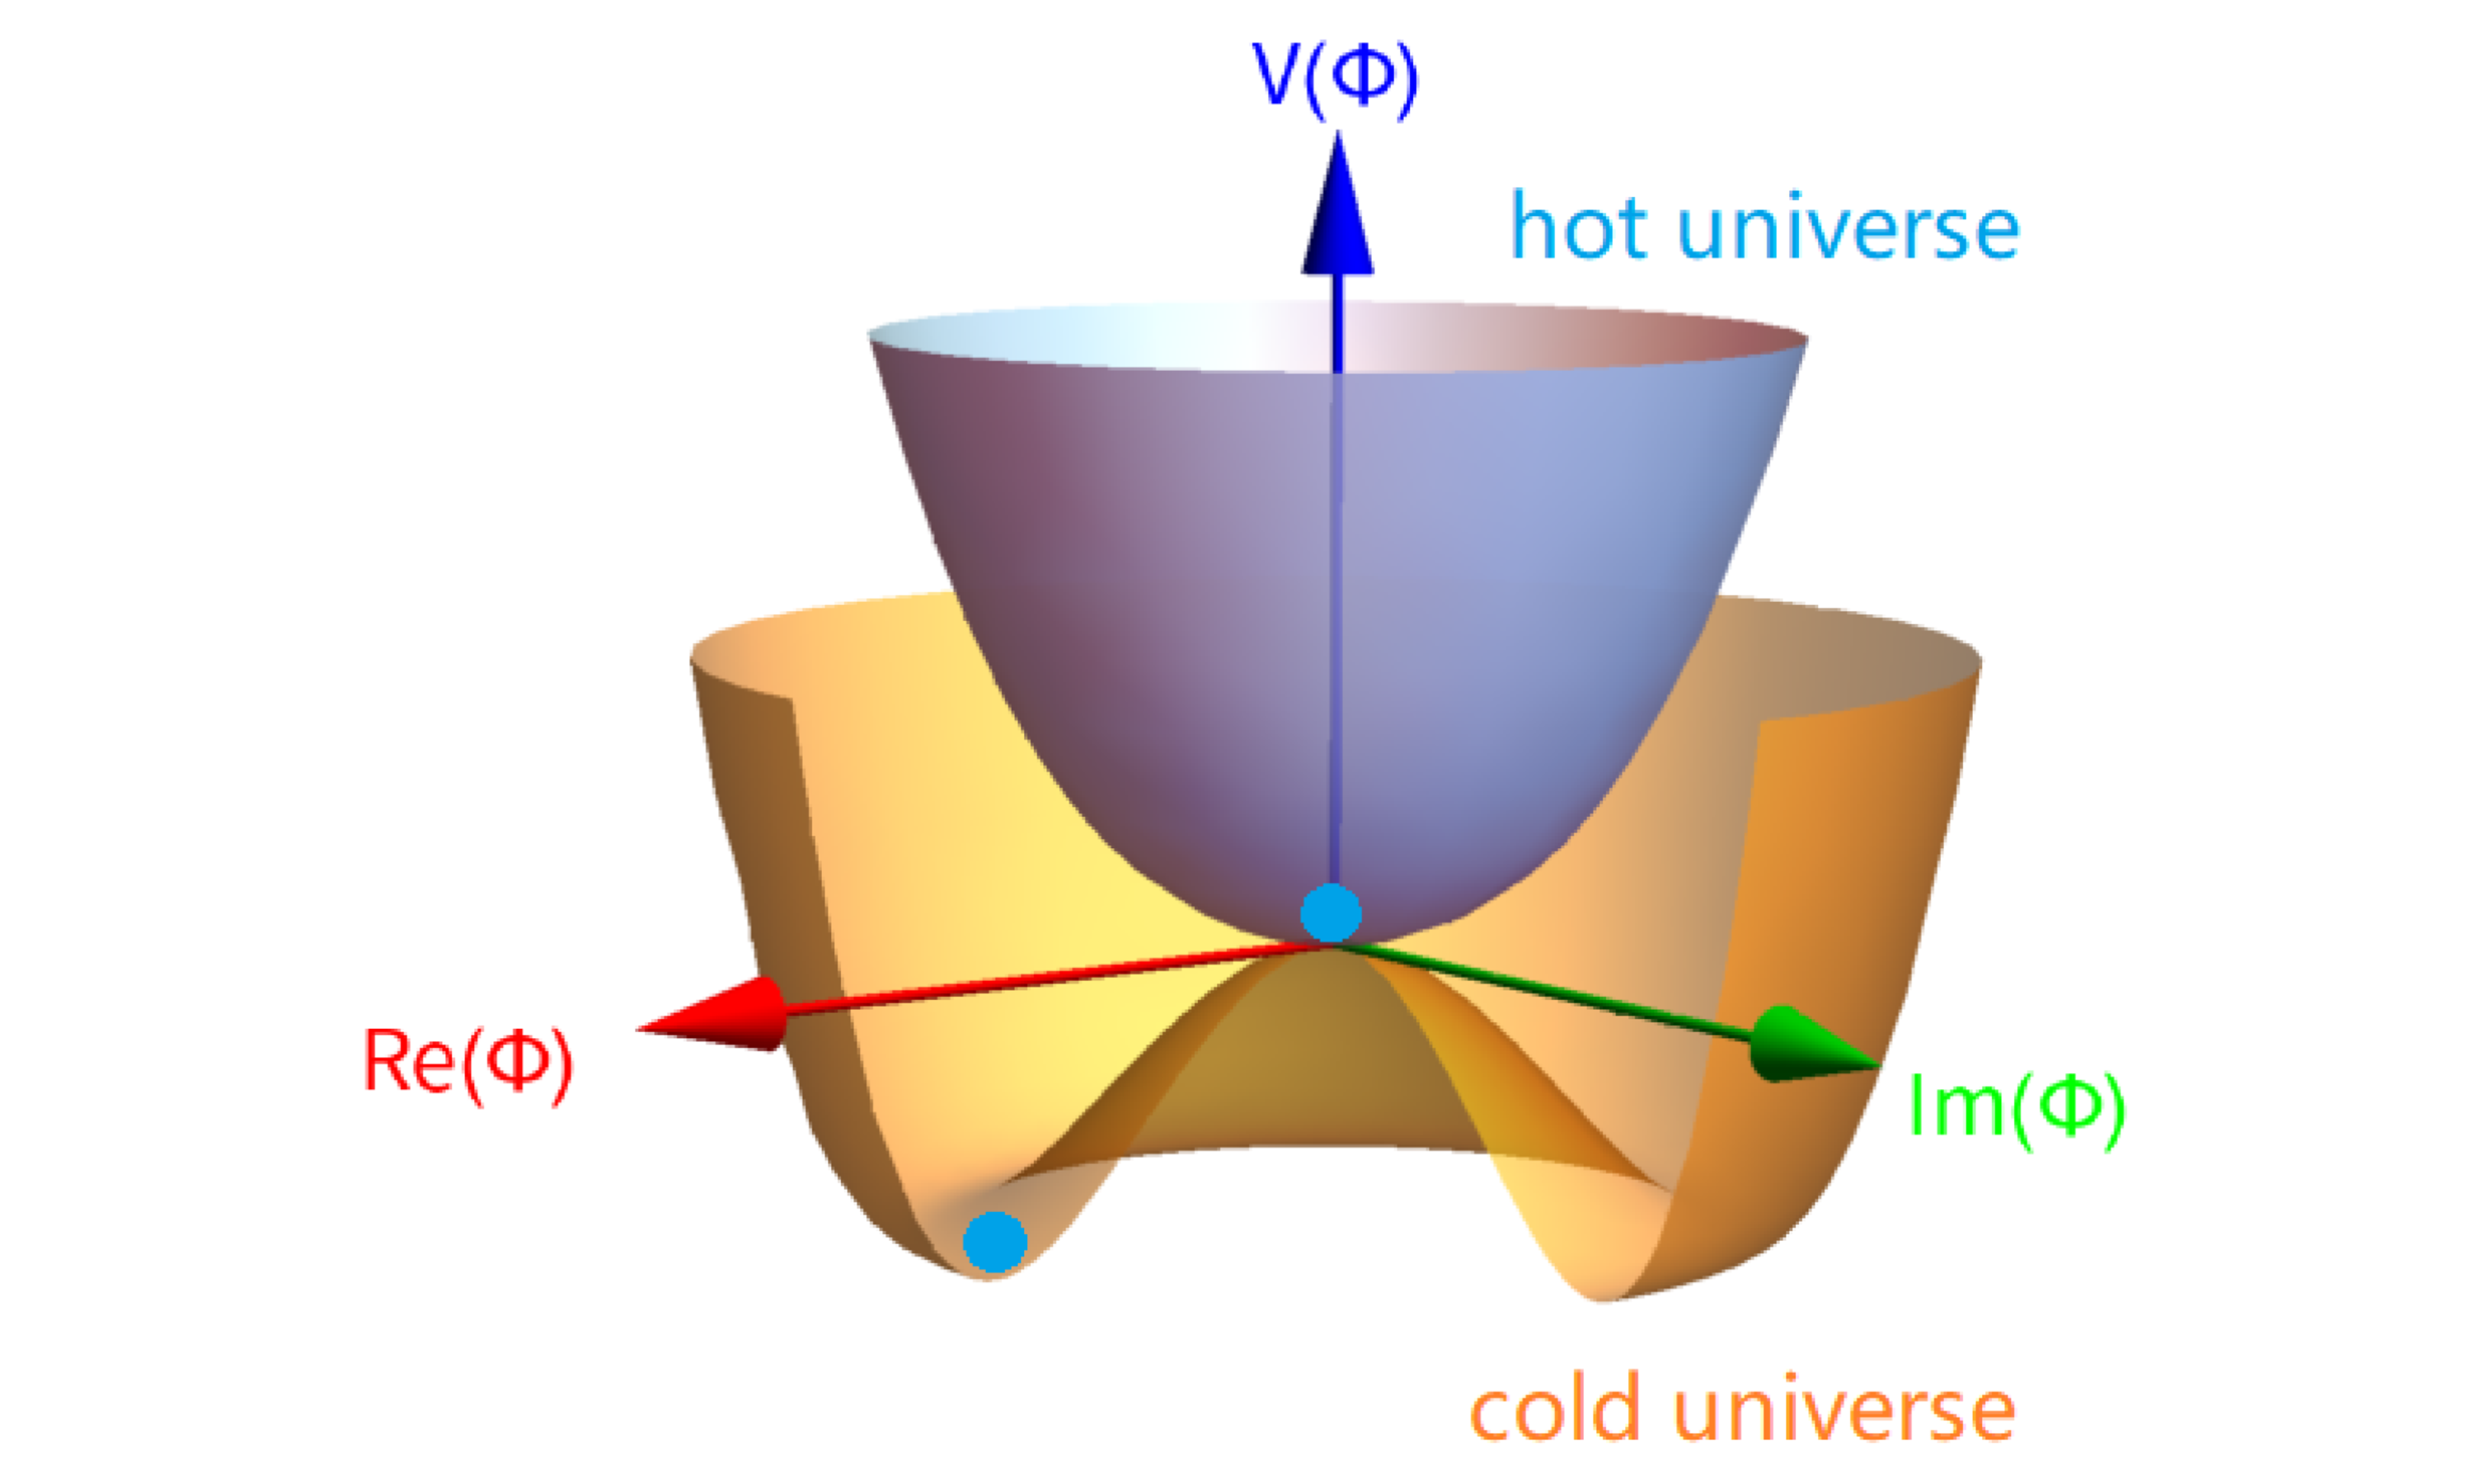
\includegraphics[width=0.7\textwidth]{figures/Part1/SM/HiggsPotential}
 \end{tabular}
 \caption{Possible shape of the Higgs potential before symmetry breaking in the hot universe (blue) and after symmetry breaking in the present universe (yellow). Adapted from~\cite{universe9040178}.}
 \label{fig:HiggsPotential}
 \end{center}
\end{figure}

Eventually, the universe cools down and $\mu^2$ becomes positive. As a consequence, an infinite number of degenerate fields arise as ground states of the potential, which corresponds to 

\begin{equation}
\phi_{min}=e^{i\varphi}\begin{pmatrix}0\\\sqrt{\mu^2/2\lambda}\end{pmatrix}\equiv\frac{e^{i\varphi}}{\sqrt{2}}\begin{pmatrix}0\\v\end{pmatrix},
\end{equation}

where $\varphi$ is the phase angle that corresponds to the choice of the degenerate field, and $v$ = 246.22 GeV~\cite{ParticleDataGroup:2022pth} is the so-called vacuum expectation value that corresponds to the physical meaning of the minimum. The ground states in this case are not invariant under \ew~symmetry. In other words, upon acquiring a vacuum expectation value by the scalar field $\phi$, the \ac{EW} symmetry will be spontaneously broken. Since the phase angle will eventually cancel out in ($\phi^{\dagger}\phi$), it is free to expand the ground-state field around the arbitrarily selected minimum $\frac{1}{\sqrt{2}}\begin{psmallmatrix}0\\v\end{psmallmatrix}$:

\begin{equation}
\phi=\frac{e^{i\hat{T}^{i}\pi^{i}(x)/v}}{\sqrt{2}}\begin{pmatrix}0\\v+h(x)\end{pmatrix},
\end{equation}

where $\hat{T}^{i}$ corresponds to the generators of the broken $SU(2)_{L}$ symmetry and $\pi^{i}(x)$ corresponds to three massless scalar bosons referred to as the Goldstone bosons~\cite{Goldstone:1962es}. The meaning of the field $h(x)$ will become clear later. The dependency on $\pi^{i}(x)$ can be removed by performing the following gauge transformation:

\begin{equation}
\phi\rightarrow\phi e^{-i\hat{T}^{i}\pi^{i}(x)/v},
\end{equation}

which corresponds to the so-called unitary gauge~\cite{Weinberg:1971fb}. Expanding the kinetic term from $\mathcal{L}_{Scalar}$,

\begin{equation}
\label{eq:ScalarKin}
(D_{\mu}\phi)^{\dagger}(D^{\mu}\phi)=\frac{1}{2}\partial_{\mu}h(x)\partial^{\mu}h(x)+(v+h(x))^2\frac{g^2}{8}[(W_{\mu}^1)^2+(W_{\mu}^1)^2+(W_{\mu}^3-\frac{g^{\prime}}{g}B_{\mu})^2].
\end{equation}

Using the relation specified in Equation~\ref{eq:CC}-\ref{eq:MixAngle}, the $v^2$ terms in Equation~\ref{eq:ScalarKin} can be rewritten as 

\begin{equation}
\begin{split}
&m_{W}^2W^{\dagger}_{\mu}W_{\mu},\\
&\frac{1}{2}m_{Z}^2Z_{\mu}Z^{\mu},
\end{split}
\end{equation}

where $m_{W}=\frac{gv}{2}$, and $m_{Z}=\frac{gv}{2\cos\theta_{\omega}}$, which corresponds to the mass of the gauge bosons W and Z, respectively. The mass of the W and Z bosons can therefore be related by $m_{Z}/m_{W}=\cos\theta_{\omega}$, which can be used to test the self-consistency of the \ac{SM}~\cite{CDF:2022hxs}. The linear combination of $v^2$ terms orthogonal to $Z_{\mu}$ cancels out and corresponds to the massless photon field:

\begin{equation}
A_{\mu}=\sin\theta_{\omega}W_{\mu}^3+\cos\theta_{\omega}B_{\mu}.
\end{equation}  

Therefore, the Z boson and photon observed at experiments can be understood as different manifestations of the same fields in the \ac{EW} theory. 

The massless gauge fields before the symmetry breaking have 2 degrees of freedom, which correspond to the two transverse polarizations. The longitudinal polarization is left empty for these massless fields because they have no rest frame when propagating in space at the speed of light. After the symmetry breaking, the $W^{\pm}_{\mu}/Z_{\mu}$ gauge fields acquire masses, which also means that they acquire longitudinal polarizations. Therefore, it can be said that the three ``would-be'' Goldstone bosons are ``eaten'' by the three gauge bosons, becoming their longitudinal components.

The remaining scalar field $h(x)$ gives rise to the only elementary scalar boson in the \ac{SM}, known as the Higgs boson. Except two mass terms for W and Z bosons, and a constant term 

\begin{equation}
\frac{1}{2}\mu^2v^2-\frac{\lambda}{2}v^4=\frac{1}{2}v^4
\end{equation}

coming from the potential, all terms in $\mathcal{L}_{Scalar}$ are related to the $h(x)$ field. They can be collected together as $\mathcal{L}_{Higgs}$:

\begin{equation}
\label{eq:LHiggs}
\begin{split}
\mathcal{L}_{Higgs}=&\frac{1}{2}\partial_{\mu}h(x)\partial^{\mu}h(x)-\frac{1}{2}m_{H}^2h(x)^2-\frac{1}{2v}m_{H}^2h(x)^3-\frac{1}{8v^2}m_{H}^2h(x)^4\\
&+[\frac{2}{v}h(x)+\frac{1}{v^2}h(x)^2](m_{W}^2W_{\mu}^{\dagger}W^{\mu}+\frac{1}{2}m_{Z}^2Z_{\mu}Z^{\mu}),
\end{split}
\end{equation}

where $m_{H}=\sqrt{2\lambda}v$. The third and fourth terms on the first line of Equation~\ref{eq:LHiggs} correspond to the Higgs triple and quartic couplings, respectively, and they come from the potential term in $\mathcal{L}_{Scalar}$. The terms on the second line of Equation~\ref{eq:LHiggs} correspond to the Higgs-Gauge boson couplings, and they come from the kinetic terms in $\mathcal{L}_{Scalar}$. The strength of these coupling is proportional to the masses of the gauge bosons. 

\section{Yukawa Interaction and Flavor Sector}
\label{sec:Flavor}

Adding Dirac mass terms $-m\bar{\psi}\psi=-m(\bar{\psi}_{L}\psi_{R}+\bar{\psi}_{R}\psi_{L})$ to the \ac{EW} theory directly will not be allowed, because they explicitly break the \ew~symmetry. Instead, the origin of the fermion masses is explained by the interaction between fermionic fields and the scalar field introduced earlier, which was first pointed out by Weinberg in his famous 1967 paper~\cite{Weinberg:1967tq}. This interaction is described by the $\mathcal{L}_{Yukawa}$ written as:

\begin{equation}
\label{eq:Yukawa}
\mathcal{L}_{Yukawa}=-(Y_{u})_{ij}\bar{Q}_{L}^{i}u_{R}^{j}\tilde{\phi}-(Y_{d})_{ij}\bar{Q}_{L}^{i}d_{R}^{j}\phi-(Y_{e})_{ij}\bar{L}_{L}^{i}e_{R}^{j}\phi + h.c.,
\end{equation}

where $Y_{f}~(f=u,d,e)$ are complex 3$\times$3 matrices, $\tilde{\phi}=i\sigma_{2}\phi^{*}$ with $\sigma_{2}$ being the second Pauli matrix. Indices i and j run over fermion generations. After the \ac{EW}~symmetry breaking, the $\mathcal{L}_{Yukawa}$ in unitary gauge becomes:

\begin{equation}
\mathcal{L}_{Yukawa}=-\frac{1}{\sqrt{2}}(v+h(x))[(Y_{u})_{ij}\bar{u}_{L}^{i}u_{R}^{j}-(Y_{d})_{ij}\bar{d}_{L}^{i}d_{R}^{j}-(Y_{e})_{ij}\bar{e}_{L}^{i}e_{R}^{j}] + h.c.,
\end{equation}

which can be rewritten as:

\begin{equation}
\mathcal{L}_{Yukawa}=-(1+\frac{h(x)}{v})[(m_{u})_{ij}\bar{u}_{L}^{i}u_{R}^{j}+(m_{d})_{ij}\bar{d}_{L}^{i}d_{R}^{j}+(m_{e})_{ij}\bar{e}_{L}^{i}e_{R}^{j}] + h.c.,
\end{equation}

where $m_f=\frac{v}{\sqrt{2}}Y_{f}~(f=u,d,e)$ is known as the fermion mass matrices. The mass matrices can be diagonalized by unitary rotations:

\begin{equation}
m_{f}=V_{f}\hat{m}_{f}W^{\dagger}_{f}~(f=u,d,e),
\end{equation}

where $\hat{m}_{f}$ are the diagonalized mass matrices. The mass term becomes:

\begin{equation}
\mathcal{L}_{mass}=-(\bar{u}_{L}V_{u}\hat{m}_{u}W_{u}^{\dagger}u_{R}+\bar{d}_{L}V_{d}\hat{m}_{d}W^{\dagger}_{d}d_{R}+\bar{e}_{L}V_{e}\hat{m}_{e}W_{e}^{\dagger}e_{R}) + h.c.
\end{equation}

Going to the so called ``mass basis'' with $u_{L}\rightarrow V_{u}u_{L}$, $u_{R}\rightarrow W_{u}u_{R}$, ...

\begin{equation}
\mathcal{L}_{mass}=-(\bar{u}_{L}\hat{m}_{u}u_{R}+\bar{d}_{L}\hat{m}_{d}d_{R}+\bar{e}_{L}\hat{m}_{e}e_{R}) + h.c.,
\end{equation}

where the diagonal elements of $\hat{m}_{f}~(f=u,d,e)$ corresponds to the Dirac mass observed in experiments. 

On the other hand, these basis transformations will affect the charged-current interactions contained in the third term of $\mathcal{L}_{gauge}$ (Equation~\ref{eq:LagGauge}):

\begin{equation}
\label{eq:LCC}
\mathcal{L}_{cc}=-\frac{g}{\sqrt{2}}[\bar{u}_{L}\gamma^{\mu}(V_{u}^{\dagger}V_{d})d_{L}+\bar{\nu}_{L}\gamma^{\mu}(V_{\nu}^{\dagger}V_{e})e_{L}]W_{\mu}^{+} + h.c, 
\end{equation}

where fermion flavor indices are suppressed, $V_{u}^{\dagger}V_{d}$ is known as the \ac{CKM} matrix~\cite{Cabibbo:1963yz,Kobayashi:1973fv}, and $V_{\nu}^{\dagger}V_{e}$ is known as the \ac{PMNS} matrix~\cite{Pontecorvo:1957cp,Maki:1962mu}. 

The \ac{CKM} matrix is a 3$\times$3 complex unitary matrix and is generally not diagonal as $V_{u}\neq V_{d}$. This enables quark flavor mixings in the charged-current interactions. For leptons, however, it is free to choose $V_{\nu}=V_{e}$ as there is no neutrino term in the $\mathcal{L}_{Yukawa}$. Therefore, the \ac{PMNS} matrix only contains diagonal elements \ac{SM} which imply the conservation of the lepton flavors.  

Looking closely at the charged-current interactions in the lepton sector:

\begin{equation}
\label{eq:LepCC}
\begin{split}
\mathcal{L}_{cc}^{lep}&=-\frac{g}{\sqrt{2}}[(\bar{\nu}_{L}^{e},\bar{\nu}_{L}^{\mu},\bar{\nu}^{\tau}_{L})\gamma^{\mu}\begin{psmallmatrix}1&0&0\\0&1&0\\0&0&1\end{psmallmatrix}(e_{L},\mu_{L},\tau_{L})^{T}]W_{\mu}^{+} + h.c.\\
&=-\frac{g}{\sqrt{2}}(\bar{\nu}_{L}^{e}\gamma^{\mu}e_{L}+\bar{\nu}_{L}^{\mu}\gamma^{\mu}\mu_{L}+\bar{\nu}_{L}^{\tau}\gamma^{\mu}\tau_{L})W^{+}_{\mu} + h.c.
\end{split}
\end{equation}

The Lagrangian is invariant under three independent global $U(1)$ symmetry, namely $U(1)_{e}\bigotimes\\U(1)_{\mu}\bigotimes U(1)_{\tau}$, which correspond to the conserved charges: family numbers of three flavors. Moreover, since the coupling strength is the same across lepton generations in Equation~\ref{eq:LepCC}, it implies that leptons of different flavors are treated equally by the weak interactions. This is the principle known as the lepton flavor universality.

It should be pointed out that the global $U(1)_{e}\bigotimes U(1)_{\mu}\bigotimes U(1)_{\tau}$ symmetry is accidental because it does not arrive by construction. Instead, it is driven by the field content of the \ac{SM}, namely the absence of right-handed neutrinos. 